\documentclass[jou]{apa6}

\usepackage[american]{babel}

\usepackage{csquotes}
\usepackage[style=apa,sortcites=true,sorting=nyt,backend=biber]{biblatex}
\DeclareLanguageMapping{american}{american-apa}
\addbibresource{bibliography.bib}


%%%%%%%%%%%%%%%%%%%%%%%%%%%%%%%%%%%%%%%%
%% Discrete Structures
%% The start of RBS stuff
%%%%%%%%%%%%%%%%%%%%%%%%%%%%%%%%%%%%%%%%

% Working internal and external links in PDF
\usepackage{hyperref}
% Extra math symbols in LaTeX
\usepackage{amsmath}
\usepackage{gensymb}
\usepackage{amssymb}
% Enumerations with (a), (b), etc.
\usepackage{enumerate}
\usepackage[framemethod=TikZ]{mdframed}
\usepackage{xcolor}
\usepackage{graphicx}
\usepackage[justification=centering]{caption}
\usepackage{fancyvrb}

\let\OLDitemize\itemize
\renewcommand\itemize{\OLDitemize\addtolength{\itemsep}{-6pt}}

\usepackage{etoolbox}
\makeatletter
\preto{\@verbatim}{\topsep=3pt \partopsep=3pt }
\makeatother

% These sizes redefine APA for A4 paper size
\oddsidemargin 0.0in
\evensidemargin 0.0in
\textwidth 6.27in
\headheight 1.0in
%\topmargin -24pt
\topmargin -32pt
\headheight 12pt
\headsep 12pt
%\textheight 9.19in
\textheight 9.35in


\title{Sample Quiz 8}
\author{Discrete Structures, Spring 2020}
\affiliation{RBS}

\leftheader{Discrete Sample Quiz 8}

\abstract{%
}

%\keywords{}

\setlength\parindent{0pt}

\begin{document}

\twocolumn

\section{Appendix: Quiz on Individual Topics}

\vspace{4pt}
{\bf Question 1.} A hacker wants to 
use {\em Arithmetic coding}
that would send a virus to the client's computer and unpack itself there.
His favorite virus uses this RNS sequence: $\textcolor{blue}{\mathtt{GACGU\$}}$, 
where $\textcolor{blue}{\mathtt{A}},\textcolor{blue}{\mathtt{C}},\textcolor{blue}{\mathtt{G}},\textcolor{blue}{\mathtt{U}}$ are four nucleobases (the useful data payload), 
but the symbol $\textcolor{blue}{\$}$ is used just once to mark 
the end of the RNS string. 

He uses the following {\em a priori} frequencies for the symbols: 

\begin{tabular}{ccccc}
$\textcolor{blue}{\mathtt{A}}$ & $\textcolor{blue}{\mathtt{C}}$ & $\textcolor{blue}{\mathtt{G}}$ & $\textcolor{blue}{\mathtt{U}}$ & $\textcolor{blue}{\mathtt{\$}}$ \\ 
$30\%$ & $10\%$ & $30\%$ & $20\%$ & $10\%$ \\
\end{tabular}


\vspace{4pt}
He starts with the half-closed line segment $S_0 = [0;1)$ and at every step (for all $i = 0,1,2,3,4,5$) creates the 
next segment $S_{i+1}$ from $S_i$ by dividing $S_i$ into five parts of lengths proportional 
to the frequencies (the proportions of subdivisions are $3\!\!:\!\!1\!\!:\!\!3\!\!:\!\!2\!\!:\!\!1$). Then $S_{i+1}$ is the
subdivision of the previous $S_i$ corresponding to the newly encoded character.
After encoding all six characters in the virus message $\textcolor{blue}{\mathtt{GACGU\$}}$, the hacker
gets the segment $S_6$.

\begin{figure}[!htb]
\center{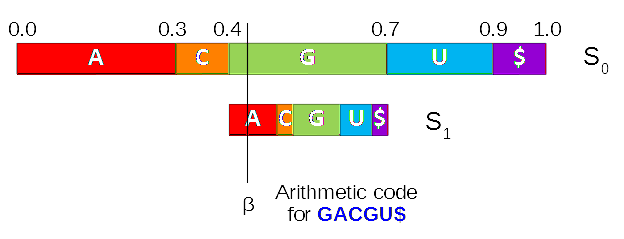
\includegraphics[width=3in]{arithmetic-coding.png}}
\caption{\label{fig:arithmetic-coding} Building arithmetic code}
\end{figure}


Find the binary fraction $\beta$ belonging to $S_6$.\\
\textcolor{teal}{\em Select one answer.}

{\bf (A)} $\beta = 0.011011101100011_2$\\
{\bf (B)} $\beta = 0.011011101100110_2$\\
{\bf (C)} $\beta = 0.011011101101001_2$\\
{\bf (D)} $\beta = 0.011011101101100_2$\\
{\bf (E)} $\beta = 0.011011101101111_2$\\


{\em Note.} In arithmetic coding any sequence of 
$n$ bits represents an interval of length $\frac{1}{2^n}$.
For example the bit sequence {\tt 010} stands for the segment of real numbers:
$[0.010_2; 0.011_2) = [0.25; 0.375)$ having length $\frac{1}{2^3} = \frac{1}{8}$. 
If the arithmetic coding yields a segment $[a;b)$ such that 
$[0.25; 0.375) \subseteq [a;b)$, then {\tt 010} is the 
result of the arithmetic coding.

The number $\beta = 0.010_2 \in [a;b)$, and the extra "0"
character ensures that the interval is not too long and it fits inside $[a;b)$. 
For example, {\tt 01} would represent a different interval $[0.25; 0.5) \neq [0.25; 0.375)$. 


\vspace{10pt}
{\bf Question 2.} We want to use a {\em regular expression} 
to find all phone numbers with the Latvian country code.
Assume that the phones can have one of the following formats (here 
symbol {\tt D} denotes any digit (0-9)). The space symbols
are used exactly as written (they are single space characters).

\begin{verbatim}
(+371) DDDDDDDD
+371 DDDDDDDD
\end{verbatim}

Pick a regular expression that would recognize just these 2 phone formats.\\
\textcolor{teal}{\em Select one answer.}


\begin{verbatim}
(A)   (+371|\(+371\)) \d{8}
(B)   (\+371|\(\+371\)) [0-9]{8}
(C)   (+371|\(+371\)) \d\d\d\d\d\d\d\d
(D)   \+371|(\+371\) [0-9]{8,8}
\end{verbatim}


{\em Note.} If you wish, you can use text editor such as Notepad++ search dialogue 
to verify which regex works. (Click {\bf Ctrl+F}, 
enter your regular expression, switch ``Search mode'' to Regular Expression, 
and click the button  ``Find All in All Opened Documents''): 


\begin{figure}[!htb]
\center{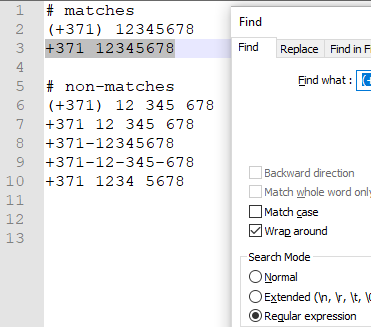
\includegraphics[width=2in]{notepad-regex.png}}
\caption{\label{fig:regex-search} Regex Search in Notepad++}
\end{figure}

If you are on a Linux machine, you can also 
test regex search with the command "grep" (and flag -E). 


\vspace{10pt}
{\bf Question 3.} About 70\% of the entries in a bit array of a {\em Bloom filter} are 
equal to $1$ as it is initialized with the words 
from some dictionary $D$. 
The Bloom filter computes $n=8$ independent hash functions to check, 
if some entry belongs to the dictionary $D$. 
What is an (approximate) chance $P$ to get a false positive?
A false positive is an event where one picks 
a random word $w \not\in D$,
and Bloom filter incorrectly states that $w$ belongs to $D$\\

\vspace{4pt}
\textcolor{teal}{\em Select one answer.}\\
{\bf (A)} $P = 30.00\%$,\\
{\bf (B)} $P = 5.76\%$,\\
{\bf (C)} $P = 3.75\%$,\\
{\bf (D)} $P = 0.66\%$.



\vspace{10pt}
{\bf Question 4.} 
A testing laboratory tests the same number of people daily, and on day $i$, the number
of people who tested positively for some health condition was $n_i$. The laboratory knows that 
the numbers $n_i$ are distributed according to {\em Poisson distribution} with the 
expected value $\lambda = 13.5$. 

By $P$ we denote the probability that on the given day 
$n_i < 5$ (i.e. less than $5$ people test 
positive for that condition). Which is the closest approximate value for this probability? 

{\bf (A)} $P = 0.26\%$,\\
{\bf (B)} $P = 0.51\%$,\\
{\bf (C)} $P = 5.78\%$,\\
{\bf (D)} $P = 10.89\%$.

{\em Note.} Another typical illustration of the same Poisson distribution: 
Imagine the ice cream ``R\={u}jienas sald\={e}jums'' with raisins. (In this case
the average number of raisins in one package is $\lambda = 13.5$; and you have to find the 
probability that a given ice cream package has at most $4$ raisins. 
See \url{https://bit.ly/2KanwIf}. 

\begin{figure}[!htb]
\center{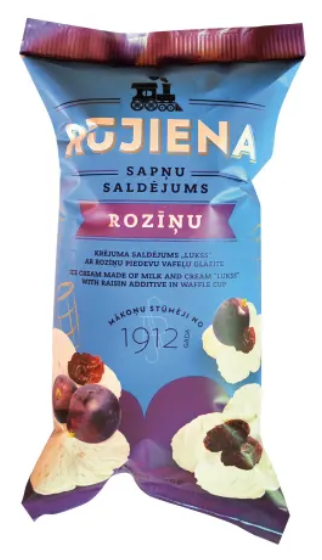
\includegraphics[width=1in]{rujiena-icecream.png}}
\caption{\label{fig:rujiena-icecream} An Ice Cream Package with Raisins satisfying Poisson Distribution}
\end{figure}


% ff <- function(k) {  return((lam^k*exp(-lam))/factorial(k) }

\vspace{10pt}
{\bf Question 5.} Find the minimum number of colors to paint the $12$ vertices
from the graph shown in Figure~\ref{fig:graph-coloring} so
that any two vertices connected with an edge are having different colors. 
(This number $n$ is called the {\em chromatic number} for the graph $G$.)

\begin{figure}[!htb]
\center{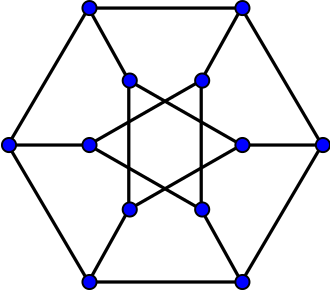
\includegraphics[width=1.6in]{durer-graph.png}}
\caption{\label{fig:graph-coloring} Graph for Vertex Coloring}
\end{figure}




\vspace{10pt}
{\bf Question 6.} Assume that the ``World Wide Web'' contains only 
$4$ pages $A,B,C,D$ that link to each other as shown in the picture below.


\begin{figure}[!htb]
\center{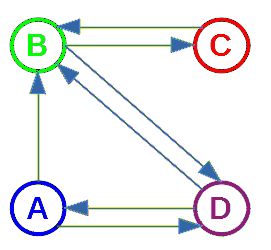
\includegraphics[width=1in]{pageranks.png}}
\caption{\label{fig:pageranks} Four webpages with links.}
\end{figure}


% https://matrix.reshish.com/multiplication.php

In the Iteration $0$ initialize the page ranks with equal values 
$$\text{PR}_0(A) = \ldots = \text{PR}_0(D) = \frac{1}{4}.$$ 
Compute the first two iterations of these pageranks, using the formulas: 
$$\left\{ \begin{array}{l}
\text{PR}_{i+1}(A) = (1 - d) + d\left( \frac{\text{PR}_i(D)}{2} \right)\\
\text{PR}_{i+1}(B) = (1 - d) + d\left( \frac{\text{PR}_i(A)}{2} + \frac{\text{PR}_i(C)}{1} + \frac{\text{PR}_i(D)}{2}  \right)\\
\text{PR}_{i+1}(C) = (1 - d) + d\left( \frac{\text{PR}_i(B)}{2} \right)\\
\text{PR}_{i+1}(D) = (1 - d) + d\left( \frac{\text{PR}_i(A)}{2} + \frac{\text{PR}_i(B)}{2} \right)
\end{array} \right.$$
Set the value of the damping factor $d=0$.

Write the values of the second iteration for all the pages:
$\text{PR}_2(A),\ldots,\text{PR}_2(D).$.

\textcolor{teal}{\em Write $4$ comma-separated numbers; round them to 
the nearest thousandth.}





\vspace{4pt}
{\em Note.} You can also use vector algebra, if you are 
familiar with multiplying matrices with vectors
\textendash{} \url{https://bit.ly/2RJTNtC}.
$$\left( \begin{array}{c}
\text{PR}_2(A)\\
\text{PR}_2(B)\\
\text{PR}_2(C)\\
\text{PR}_2(D)
\end{array} \right) = \left( 
\begin{array}{cccc}
\textcolor{blue}{0}   & \textcolor{green}{0}   & \textcolor{red}{0} & \textcolor{purple}{1/2} \\
\textcolor{blue}{1/2} & \textcolor{green}{0}   & \textcolor{red}{1} & \textcolor{purple}{1/2} \\
\textcolor{blue}{0}   & \textcolor{green}{1/2} & \textcolor{red}{0} & \textcolor{purple}{0} \\
\textcolor{blue}{1/2} & \textcolor{green}{1/2} & \textcolor{red}{0} & \textcolor{purple}{0}
\end{array} \right)^2 \cdot \left( \begin{array}{c}
1/4 \\
1/4 \\
1/4 \\
1/4
\end{array} \right).$$
In this formula a square matrix $4 \times 4$ is twice multiplied to a $4 \times 1$
vector $(1/4, 1/4, 1/4, 1/4)$ from the left side. 
%See \url{https://bit.ly/2VkZHnh}. 


\vspace{4pt}
{\em Note.} \url{https://checkpagerank.net/check-page-rank.php}
shows that:\\
{\tt https://www.bitl.lv/} has PageRank $2/10$,\\
{\tt https://www.delfi.lv/} has PageRank $6/10$.\\
This does {\bf not} mean that there are three times more 
inbound links to Delfi than to BITL (or that these links are three times more ``valuable''). 
The value returned by this web resource is a {\em logarithmic measure}
of its iterative value. In fact, the difference between $2/10$ and $6/10$
means that the popularity of these pages differs by many orders of magnitude. 
See \url{https://bit.ly/2yrRMf7}.


\vspace{10pt}
{\bf Question 7.} As you probably know, {\em Karatsuba's algorithm} can express 
the multiplication of two numbers of length $n$ digits as 
three multiplications of numbers of length $n/2$ (i.e. the number of 
operations are three times larger, but the operands become two times shorter). 
This ultimately means that Karatsuba's algorithm requires
only $O(n^{1.585})$ operations to multiply numbers of length $n$.

Imagine that somebody has invented a new operation $a \otimes b$ for 
some objects $a,b$ (both $a,b$ have the same size $n$). 
Assume that s/he knows how to express 
$a \otimes b$ using $7$ operations $a_i \otimes b_i$ (where $i = 1,2,\ldots,7$, and
all $a_i,b_i$ have size $n/2$, i.e. half the size of the original operands $a,b$). 
({\em We do not care, what the operation $\otimes$ does; but we know that we 
can compute it for arguments $a,b$ of length $1$ in constant time; it is 
therefore easy for very short arguments.})

Find the best Big-O-Notation estimate for the time needed to compute $a \otimes b$, if $a,b$ are
both of size $n$. 

{\bf (A)} $O(n^2)$\\
{\bf (B)} $O(n^2 \log n)$\\
{\bf (C)} $O(n^{2.646})$\\
{\bf (D)} $O(n^{2.808})$\\
{\bf (E)} $O(n^3)$\\
{\bf (F)} $O(n^3 \log n)$\\
\textcolor{teal}{\em Select one answer.}

\vspace{4pt}
{\em Note 1.} One can use Master's theorem (Rosen2019, p.558) for 
this problem and also for the Karatsuba's algorithm.

\vspace{4pt}
{\em Note 2.} If the algorithm falls in multiple Big-O complexity classes, pick 
the one that shows the slowest growth. For example, if a speed of an algorithm is 
both in $O(n^2)$ and $O(n^3)$, 
then $O(n^2)$ would be a more precise and a more useful estimate.


\vspace{10pt}
{\bf Question 8.} Assume that two players $A$ and $B$ play a {\em matrix game}. 
They simultaneously guess one number each. Either player can guess 
one of these three numbers: $\{ 1,2,5 \}$. 
The payoff matrix is shown below. 
In each cell the first number is what is paid to player $A$, 
the second number is paid to player $B$. 

\begin{figure}[!htb]
\center{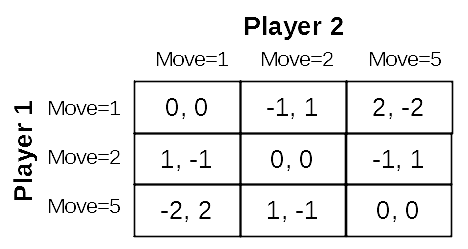
\includegraphics[width=2.4in]{matrix-game.png}}
\caption{\label{fig:matrix-game} Matrix game with payoffs.}
\end{figure}

Expressed in human language, the rules are as follows. 
Assume that the player $A$ just guessed a number $a$, and player $B$ guessed 
a number $b$. 
\begin{itemize}
\item If $a=b$, then it is a tie; nobody pays anything.
\item If $a>b$ (yet $a < 3b$), then $B$ pays to $A$ one euro. (And also, 
if $b>a$ yet $b < 3a$, then $A$ pays to $B$ one euro.)
\item If $a \geq 3b$, then $A$ pays to $B$ two euros. (And also, if $b \geq 3a$, 
then $B$ pays to $A$ two euros.)
\end{itemize}

{\em In this number guessing game one can win by guessing a number which is a little
bit larger than the other player's number. But one should not guess a number which is 
larger than the other by ``a lot'' (if you exceed the other player's number
three times or more, then you suffer a double loss.).}

Which can be {\em Nash equilibrium} for this number guessing game?
(You can assume that one of the answer variants is correct \textendash{} 
the same optimal strategy for both players. It is enough to find the 
one that beats all the other strategies.) 
Each strategy lists the probabilities for guessing the number $x$: 

{\bf (A)} $P(x = 1) = 1/3$, $P(x = 2) = 1/3$, $P(x = 5) = 1/3$.\\
{\bf (B)} $P(x = 1) = 0$, $P(x = 2) = 1/2$, $P(x = 5) = 1/2$.\\
{\bf (C)} $P(x = 1) = 1/2$, $P(x = 2) = 1/2$, $P(x = 5) = 0$.\\
{\bf (D)} $P(x = 1) = 1/4$, $P(x = 2) = 1/2$, $P(x = 5) = 1/4$.\\
{\bf (E)} $P(x = 1) = 2/6$, $P(x = 2) = 3/6$, $P(x = 5) = 1/6$.\\
\textcolor{teal}{\em Select one answer.}


\vspace{10pt}
{\bf Question 9.} The first iterations using Lindermayer system are given:\\
{\bf Iteration 0:} {\tt A}\\
{\bf Iteration 1:} {\tt AB}\\
{\bf Iteration 2:} {\tt ABBA}\\
{\bf Iteration 3:} {\tt ABBABAAB}\\
{\bf Iteration 4:} {\tt ABBABAABBAABABBA}

({\em To get Iteration 5: Take Iteration 4, 
change all A's into B's and
vice versa, and append such string to the end of Iteration 4.})
Find the correct set of rules to generate this L-system. 

{\bf (A)} ${\displaystyle \left\{ \begin{array}{l}
\mathtt{A} \rightarrow \mathtt{B}\\
\mathtt{B} \rightarrow \mathtt{BA}
\end{array} \right. }$\\
{\bf (B)} ${\displaystyle \left\{ \begin{array}{l}
\mathtt{A} \rightarrow \mathtt{AB}\\
\mathtt{B} \rightarrow \mathtt{AA}
\end{array} \right. }$\\
{\bf (C)} ${\displaystyle \left\{ \begin{array}{l}
\mathtt{A} \rightarrow \mathtt{AB}\\
\mathtt{B} \rightarrow \mathtt{BA}
\end{array} \right. }$\\
{\bf (D)} ${\displaystyle \left\{ \begin{array}{l}
\mathtt{A} \rightarrow \mathtt{AB}\\
\mathtt{B} \rightarrow \mathtt{AB}
\end{array} \right. }$

\textcolor{teal}{\em Select one answer.}

{\em Note.} We can have a {\em turtle} that reads this 
sequence and performs actions:
\begin{itemize}
\item Letter $\mathtt{A}$: Step $1$ unit ahead, turn 
$60^{\circ}$ counterclockwise.
\item Letter $\mathtt{B}$: Turn $180^{\circ}$. 
\end{itemize}
In this case the iterations $0,2,4,\ldots$ would produce
a fragment of Koch snowflake (Figure~\ref{fig:lindenmayer-system}).

\begin{figure}[!htb]
\center{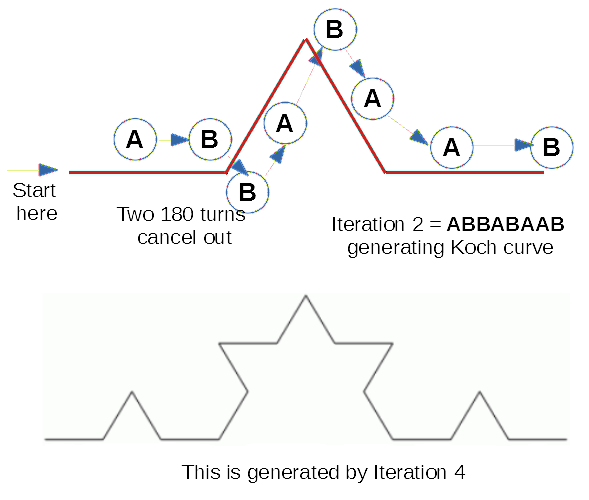
\includegraphics[width=2.5in]{lindenmayer-system.png}}
\caption{\label{fig:lindenmayer-system} Koch curve as an L-system}
\end{figure}





\vspace{10pt}
{\bf Question 10.} Assume that someone uses
a {\em secure hash} algorithm $h(x)$ that for any file $x$
outputs a hash value consisting of exactly $100$
bits. (The typical SHA-256 algorithm would return $256$ bits.)

Assume that we want to use brute force to find 
hash collision \textendash{} two different files $x_1,x_2$
such that $h(x_1) = h(x_2)$. 
You can estimate, how many hash values we need to compute before we 
get at least $50\%$ probability to find a hash collision. 
Estimation can be done using Square aproximation from 
the Birthday paradox: 
\begin{equation}
\label{eq:square-approximation}
p_{\text{collision}} \approx \frac{n^2}{2m},
\end{equation}
Formally: If a hash function $h(x)$ can take $m$ different values and
we randomly pick $n$ different integer numbers $x_1,\ldots,x_n$, then the probability 
that there is at least one collision ($h(x_i) = h(x_j)$ and $x_i \neq x_j$) is approximately expressed by
the formula (\ref{eq:square-approximation}). See \url{https://bit.ly/2RNjhGB}.

Assume that a single hash value $h(x)$ can be computed in one microsecond
($1\,\mu{}s = 10^{-6}\,s$). Estimate the number of years it would take to produce a
collision for a 100-bit secure hash algorithm with probability at least $50\%$. 

{\bf (A)} The expected time is $0.11$ years.\\
{\bf (B)} The expected time is $35.7$ years.\\
{\bf (C)} The expected time is $71.4$ years.\\
{\bf (D)} The expected time is $856$ years.\\
{\bf (E)} The expected time is $4.02\cdot 10^{16}$ years.\\
\textcolor{teal}{\em Select one answer.}


\vspace{10pt}
{\bf Question 11.} Consider the following 
problem solving strategies: 

{\footnotesize
{\bf (A)} {\bf Drawing a picture.} Can you 
write down all the things you need to consider on paper? 
Can you order them nicely in a list or a table? 
Can you show them in a two-dimensional or a three-dimensional drawing?\\
{\bf (B)} {\bf Getting hands dirty.} Can you start experimenting with the 
problem, plug in specific values, see where they lead you?\\
{\bf (C)} {\bf Going to the extremes.} Can you pick some ``borderline case''?
Is there the smallest or the largest item that is possible in the problem?\\
{\bf (D)} {\bf Lateral thinking.} Could it happen that your current solving approach 
is not applicable or is too inefficient? Can you pretend that you 
have not spent many years studying mathematics at school; 
can you apply lateral/divergent thinking out of the box to 
come up with something unexpected?\\
{\bf (E)} {\bf Looking for symmetries.} Can we switch two numbers or two letters in our 
notation? Can we inspect just one item and notice that many others are identical?\\
{\bf (F)} {\bf Making it easier.} Can we make a simpler version of this problem and
solve it first? Insert a smaller number? Solve only one particular case of it?\\
{\bf (G)} {\bf Penultimate step.} What precondition must take place before 
the final solution step is possible? Imagine, which result you would need 
in order to say that you are ``almost done''.\\
{\bf (H)} {\bf Wishful thinking.} Can you apply some outrageous simplification to your 
initial problem. Imagine for a while that you have already solved it: What would that imply?
% http://courses.cs.vt.edu/~cs4104/shaffer/Fall2010/PSintro.pdf
}

Now consider the following problem:

\begin{figure}[!htb]
\center{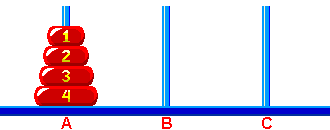
\includegraphics[width=2in]{tower-of-hanoi.png}}
\caption{\label{fig:tower-of-hanoi} Tower of Hanoi}
\end{figure}

\begin{mdframed}[roundcorner=6pt]
{\footnotesize
{\bf Problem.} A Tower of Hanoi (Figure~\ref{fig:tower-of-hanoi}) 
has three pegs ($A$, $B$, $C$) and
four disks initially on the peg $A$. The task is to move all the four disks to the peg $B$, where
the following rules apply:\\
Rule 1: Only one disk can be moved at a time.\\
Rule 2: Each move consists of taking the upper disk from any peg and moving it to 
another peg.\\
Rule 3: No larger disk may be placed on top of a smaller disk.

{\em The solver wants to come up with the sequence of moves. S/he has tried
a similar game with just three disks with some trial and error, but 
is not sure how to proceed in the case with four disks. Somebody suggests 
a few ``natural looking'' hints.}

{\bf Hint 1.} Find the disk that is the hardest to move anywhere or moved least frequently?\\
{\bf Hint 2.} To which peg all the other disks need to go before we move this disk?\\
{\bf Hint 3.} Assume that you know how to move three disks from the peg $A$ to the peg $B$. 
Can you move them between any other pegs? How?
}
\end{mdframed}


What kind of problem solving strategies are contained in the hints?

\textcolor{teal}{\em Select up to three relevant strategies (A-H).}



\begin{center}
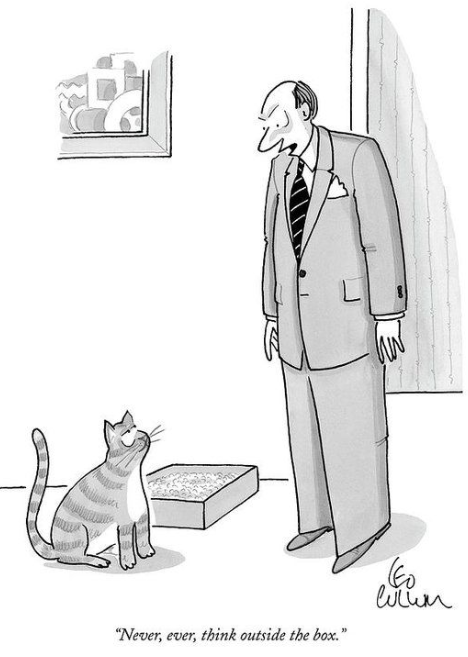
\includegraphics[width=2in]{thinking-outside-the-box.png}\\
\textcopyright{} {\em Leo Cullum}, \url{https://www.newyorker.com/}
\end{center}

\vspace{10pt}
{\bf Question 12.} Someone wants to compute a MD5 checksum for the following file: 

\textcolor{blue}{
{\tt 95.211.48.179~~~bitl.lv}
}

The following is true: 
\begin{itemize}
\item File {\tt hosts.txt} is exactly $23$ bytes long.
\item The IP address is seperated from {\tt bitl.lv} by 
a single horizontal tab (byte in hexadecimal: {\tt 0x09}). 
\item The only line is ends with a Windows-style line ending (carriage return, line feed: 
bytes in hexadecimal: {\tt 0x0D}, {\tt 0x0A}). 
\end{itemize}

Figure~\ref{fig:hosts-file} shows file displayed by {\em Total Commander}; 
button {\bf F3}, then menu item {\bf Options $>$ Hex} (and also in the Notepad++ editor).

\begin{figure}[!htb]
\center{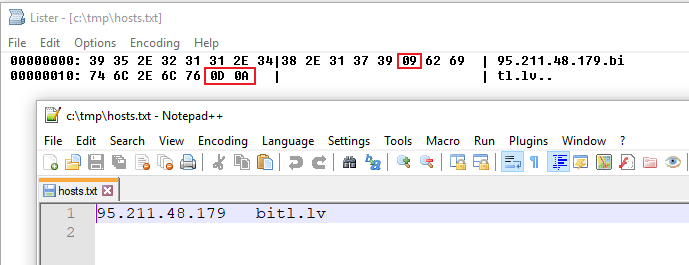
\includegraphics[width=3in]{hosts-file.png}}
\caption{\label{fig:hosts-file} Bytes in file {\tt hosts.txt}}
\end{figure}

\textcolor{teal}{\em Copy the whole MD5 checksum in your answer.}

{\em Note.} In this exercise it is important to have exactly the
same file content as shown in the picture. 
For example, replacing the {\bf TAB} character
by one or more spaces (or Windows-style line ending with a UNIX-style
line ending) would totally change MD5. 
(For secure hashes there is absolutely no string tokenization \textendash{}
unlike plagiarism detection they are very sensitive against
the smallest changes in their input.)


\vspace{10pt}
{\bf Question 13.} There are two people playing a game: Player $A$ (he is the Maximizer \textendash{} wants
to go down to a leaf with maximum payoff), and Player $B$ (he is the Minimizer \textendash{} wants
to minimize the $A$'s payoff). The current position is the root of the tree (Figure~\ref{fig:minimax}) and it is Player's $A$
turn to make the first move (to any of the root's children). After that Player $B$ moves (going down one more level) and so on
\textendash{} until they reach a leaf, which shows the payoff for Player $A$.\\
Find the maximum payoff for Player $A$ (you could use minimax algorithm with or without Alpha-Beta pruning 
speedup to find out). 

\textcolor{teal}{\em Write the payoff as a positive integer.}

\begin{figure}[!htb]
\center{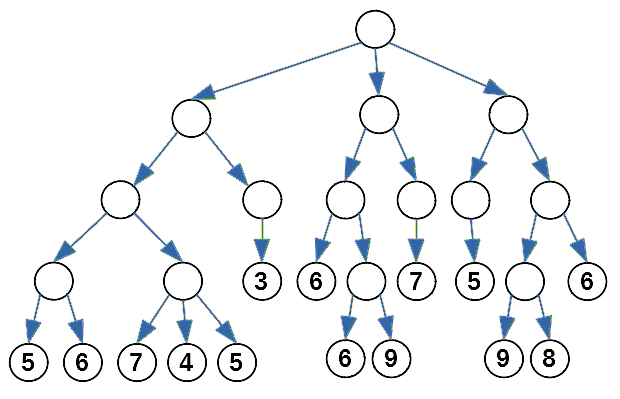
\includegraphics[width=3in]{minimax.png}}
\caption{\label{fig:minimax} Game positions in a tree.}
\end{figure}


\vspace{10pt} 
{\bf Question 14.} If you verify the Conway's game of life the configuration $P_0$ 
of a straight line with $4$ live cells (Figure~\ref{fig:conway}), 
you need $N = 2$ steps until you reach ``periodic state'' $P_2$ that will 
return after period $T = 1$ (i.e.\ returning needs just one step $P_3 = P_2$, 
since ``beehive'' configuration is stable). So in this case $(N,T)=(2,1)$ \textendash{}
there are $N=2$ preliminary steps, and after that there is a period of length $T=1$. 

\begin{figure}[!htb]
\center{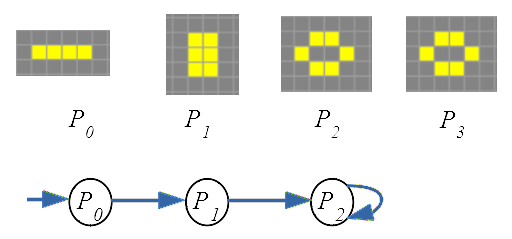
\includegraphics[width=2.2in]{conway.png}}
\caption{\label{fig:conway} Conway game for a line of $4$.}
\end{figure}

Now consider a different starting position $P_0$ that contains a straight line 
of $5$ live cells (Figure~\ref{fig:conway2}). Determine the number of steps $N$ needed
to reach the first position $P_N$ that would repeat infinitely often, and
the length of period $T$ with which the subsequent steps repeat, i.e. 
the smallest positive integer $T$ with the property:
$$\forall k \in \mathbb{Z}_{0+},\;(k \geq N)\;\rightarrow\; (P_{k+T} = P_k).$$

\begin{figure}[!htb]
\center{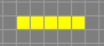
\includegraphics[width=0.6in]{conway2.png}}
\caption{\label{fig:conway2} Starting position $P_0$ for a line of $5$.}
\end{figure}

\textcolor{teal}{\em Write two comma-separated integers $N,T$.}

{\em Note.} In Conway's game there are some positions 
that are not periodic (glider guns that 
constantly create new stuff), but most simple positions eventually reach periodic state. 
Therefore the numbers $N$ and $T$ are defined in these cases.




\vspace{10pt} 
{\bf Question 15.} A mathematical theory $\mathcal{T}$ (in a similar way as Coq software) 
provides rules to prove various mathematical statements. 
Assume that in this theory $\mathcal{T}$ one can prove some statement $A$ and also the
statement $\neg A$. Which description is true for this theory:

{\bf (A)} $\mathcal{T}$ is consistent.\\
{\bf (B)} $\mathcal{T}$ is not consistent.\\
{\bf (C)} $\mathcal{T}$ is complete.\\
{\bf (D)} $\mathcal{T}$ is not complete.\\
{\bf (E)} $\mathcal{T}$ is effectively axiomatized.\\
{\bf (F)} $\mathcal{T}$ is not effectively axiomatized.\\
\textcolor{teal}{\em Select one answer.}


\vspace{10pt} 
{\bf Question 16.} Some banks can issue
19-digit credit card numbers (instead of the more typical 16-digit ones). 
Assume that there is a 19-digit number that satisfies the Luhn check (mod $10$):

$$\mathtt{557367054456450571\ast}.$$

Please find the digit that is written in the place of the last $\ast$ symbol.

\textcolor{teal}{\em Write a single digit.}


\vspace{10pt} 
{\bf Question 17.} 
Some text $T$ has been tokenized into a sequence of $N$ words ($w_0,\ldots,w_{N-1}$). 
Assume that you assigned
unique numbers to the stemmed words (each word $w_i$ in the text $T$ is replaced by 
a number $n(w_i)$); and then computed rolling hash values for 
five consecutive words in this text using this formula:\\

%\begin{align}
% & H(w_1,w_2,w_3,w_4,w_5) = \nonumber \\
%= & \left( n(w_1) \cdot a^4 + n(w_2) \cdot a^3 + n(w_3) \cdot a^2 + \right. \nonumber \\
%+ & \left. n(w_4) \cdot a^1 + n(w_5) \cdot a^0 \right)\;\; \text{mod}\;\; q. \nonumber
%\end{align}

{\footnotesize
\begin{align}
 & H(w_1,w_2,w_3,w_4,w_5) = \nonumber \\
= & \left( n(w_1) \cdot a^4 + n(w_2) \cdot a^3 + n(w_3) \cdot a^2 + n(w_4) \cdot a^1 + n(w_5) \right)\, \text{mod}\,q. \nonumber
\end{align}
}


This is a polynomial value for the argument $a$ followed by a remainder when dividing by $q$.
Parameters $a$ and $q$ are two large primes.

We compute all such hash values:
$$\left\{ \begin{array}{l}
v_0 = H(w_0,w_1,w_2,w_3,w_4),\\
v_1 = H(w_1,w_2,w_3,w_4,w_5),\\
\ldots\\
v_{N-5} = H(w_{N-5},w_{N-4},w_{N-3},w_{N-2},w_{N-1}).
\end{array} \right.$$

It turned out that $10\%$ of these hash values were found in an existing
hashtable $H$ (built from some existing texts using the same hash function) \textendash{}
about $5\%$ of the values in that hashtable are marked (the others are empty).
What is the most likely explanation for this? 

{\bf (A)} Text $T$ contains large chunks of text that is copy-pasted from other sources.\\
{\bf (B)} Overlaps of the size $10\%$ can happen by chance. On the other hand, overlaps
exceeding $1/5$ (the size of the rolling hash window) would be highly unusual and 
would require manual inspection.\\
{\bf (C)} This is not an effective way to detect copying and plagiarism.
Rolling hash should instead run on characters (not entire words),
since multiple authors may use the same words.\\
\textcolor{teal}{\em Select one answer.}





\vspace{10pt} 
{\bf Question 18.} Jane took an ordinary soccer ball made from an elastic material
(Figure~\ref{fig:icosahedron3d}).


\begin{figure}[!htb]
\center{
\includegraphics[width=2in]{truncated-icosahedron-3d.png}
\caption{\label{fig:icosahedron3d} 3D Soccer Ball}
}
\end{figure}


She stretched one of its faces so that it became a planar graph
(Figure~\ref{fig:icosahedron2d}).
Then she marked a Hamiltonian cycle in this graph (not shown).


\begin{figure}[!htb]
\center{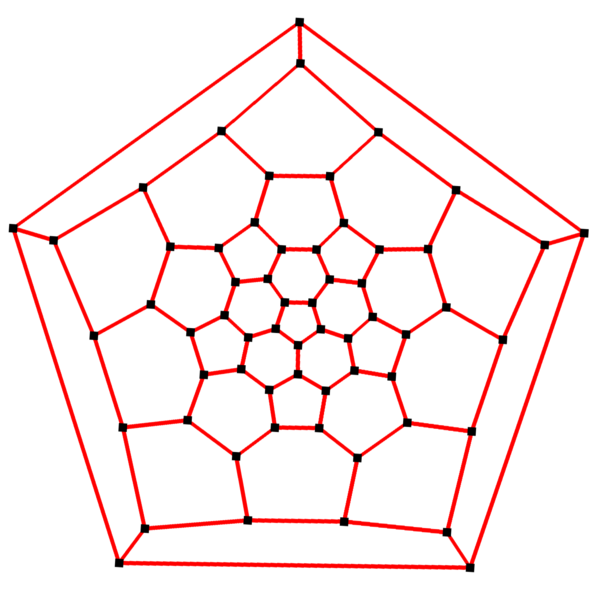
\includegraphics[width=2.4in]{truncated-icosahedron.png}}
\caption{\label{fig:icosahedron2d} Planar Soccer Ball}
\end{figure}

How many edges of this graph do {\bf not} belong to the Hamiltonian cycle?\\
\textcolor{teal}{\em Write a positive number.}


\mbox{}
\newpage

\subsection{Answers}

\vspace{4pt}
{\bf Question 1.} Answer {\bf (D)}\\
The intervals encoding the string $\textcolor{blue}{\mathtt{"GACGU\$"}}$
form the following sequence: 
$$\left\{ \begin{array}{l}
S_0 = [0.000000; 1.000000]\;\text{encodes}\;\textcolor{blue}{\mathtt{""}}\;\text{(empty string)}, \\
S_1 = [0.400000; 0.700000]\;\text{encodes}\;\textcolor{blue}{\mathtt{"G"}}, \\
S_2 = [0.400000; 0.490000]\;\text{encodes}\;\textcolor{blue}{\mathtt{"GA"}}, \\
S_3 = [0.427000; 0.436000]\;\text{encodes}\;\textcolor{blue}{\mathtt{"GAC"}}, \\
S_4 = [0.430600; 0.433300]\;\text{encodes}\;\textcolor{blue}{\mathtt{"GACG"}}, \\
S_5 = [0.432490; 0.433030]\;\text{encodes}\;\textcolor{blue}{\mathtt{"GACGU"}}, \\
S_6 = [0.432976; 0.433030]\;\text{encodes}\;\textcolor{blue}{\mathtt{"GACGU\$"}}. \\
\end{array} \right.$$

To make the sequence of intervals $S_0 \supset S_1 \supset \ldots \supset S_6$, 
we can define iterative sequences $\text{Left}_i$, $\text{Length}_i$ describing 
the left endpoint and the length of each successive interval so that for every 
$i = 0,1,\ldots,6$: 
$$S_i = \left[ \text{Left}_i; \text{Left}_i + \text{Length}_i \right].$$

These sequences are defined in terms of the offsets and frequencies 
of the characters $c_0, c_1, \ldots, c_5$. 

$$\left\{ \begin{array}{l}
\text{Left}_{i+1} = \text{Left}_{i} + \text{Left}_{i} \cdot \text{Offset}(c_i) \\
\text{Length}_{i+1} = \text{Length}_{i}  \cdot \text{Frequency}(c_i) \\
\end{array} \right.$$

For each encodable character the offsets and frequencies are defined in this table:

\begin{tabular}{|l|l|l|} \hline
Character & Frequency & Offset \\ \hline
$\mathtt{A}$ & $0.3$ & $0.0$ \\ \hline
$\mathtt{C}$ & $0.1$ & $0.3$ \\ \hline
$\mathtt{G}$ & $0.3$ & $0.4$ \\ \hline
$\mathtt{U}$ & $0.2$ & $0.7$ \\ \hline
$\mathtt{\$}$ & $0.1$ & $0.9$ \\ \hline
\end{tabular}

The only binary number $\beta$ that belongs to 
$S_6 = [0.432976; 0.433030]$ is shown in answer {\bf (D)}:
$$\beta = 0.011011101101100_2 = 0.4329834_{10}.$$


\vspace{10pt}
{\bf Question 2.} Answer {\bf (B)}\\
The only syntactically correct regular expression is 
\begin{verbatim}
(\+371|\(\+371\)) [0-9]{8}
\end{verbatim}

\vspace{10pt}
{\bf Question 3.} Answer {\bf (B)}\\
The probability that all $8$ hash values 
will happen to be $1$ is 
$$0.7^8 = 0.05764801.$$



\vspace{10pt}
{\bf Question 4.} (None of the answers is right)\\
We can add up the probabilities, using Poisson distribution formula: 
$$P(X = k) = \frac{\lambda^k \cdot e^{-\lambda}}{k!}.$$
By adding up the first $5$ values of this distribution we get this expression with $\lambda = 13.5$: 
$$P(X < 5) = \sum\limits_{k=0}^{4} \frac{\lambda^k \cdot e^{-\lambda}}{k!} \approx 0.000707.$$ 
Therefore the probability to get less than $5$ raisins is $0.0707\%$. 

Since all the answer variants were wrong, everyone gets full credit for this.




\vspace{10pt}
{\bf Question 5.} Answer: $3$\\
Three colors are sufficient as shown in the picture. 
But two colors are impossible (since the graph contains a triangle \textendash{}
a full graph $K_3$). 

\begin{figure}[!htb]
\center{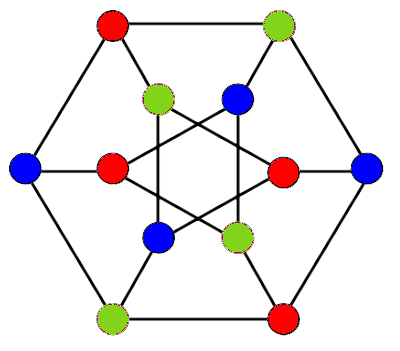
\includegraphics[width=1.5in]{durer-graph-colored.png}}
\caption{\label{fig:durer-graph-colored} D\"{u}rer Graph colored in $3$ colors.}
\end{figure}

This graph is planar (you can draw it without intersecting edges); 
it also has a famous 
polyhedron (D\"{u}rer solid); it was shown in an engraving 
made in 1514 called {\em Melencolia I}. See
\url{https://bit.ly/2KE2QZl}. 



\vspace{10pt}
{\bf Question 6.} Answer: $0.125,0.313,0.250,0.313$\\
We write the vectors as they are multiplied with the 
$4 \times 4$ matrix. The components in the vector 
correspond to the pageranks (iterations $0$, $1$ and $2$). 
$$v_0 =  \left( \begin{array}{c}
1/4 \\
1/4 \\
1/4 \\
1/4 \\
\end{array} \right);\;\;
v_1 = \left( \begin{array}{c}
1/8 \\
1/2 \\
1/8 \\
1/4 \\
\end{array} \right);\;\;
v_2 = \left( \begin{array}{c}
1/8 \\
5/16 \\
1/4 \\
5/16 \\
\end{array} \right).$$

\vspace{10pt}
{\bf Question 7.} Answer {\bf (D)}\\
The time complexity of such algorithm is $O(n^{\log_2 7})$ by Master's theorem. Since 
$\log_2 7 \approx 2.807355 < 2.808$, we have the time complexity in $O(n^{2.808})$ (it is the best estimate that is given 
among the arguments).


\vspace{10pt}
{\bf Question 8.} Answer {\bf (D)}\\
Since we can assume that one of the five strategies is optimal, it is sufficient to compare the strategies. 
We assume that Players $A$ and $B$ adopt one of the five suggested strategies
plus one more simple strategy {\bf (F)} (always guess number $2$). 

There are altogether $36$ variants. 
For each pair of strategies we compute the payoff for the Player $A$. 
We want to find the strategy for Player $A$ 
that beats any strategy chosen by $B$ (or at least achieves a tie). 

{\bf (A)} $P(x = 1) = 1/3$, $P(x = 2) = 1/3$, $P(x = 5) = 1/3$.\\
{\bf (B)} $P(x = 1) = 0$, $P(x = 2) = 1/2$, $P(x = 5) = 1/2$.\\
{\bf (C)} $P(x = 1) = 1/2$, $P(x = 2) = 1/2$, $P(x = 5) = 0$.\\
{\bf (D)} $P(x = 1) = 1/4$, $P(x = 2) = 1/2$, $P(x = 5) = 1/4$.\\
{\bf (E)} $P(x = 1) = 2/6$, $P(x = 2) = 3/6$, $P(x = 5) = 1/6$.\\
{\bf (F)} $P(x = 1) = 0$, $P(x = 2) = 1$, $P(x = 5) = 0$.\\

The strategies of Player $A$ are shown in rows; strateges of Player $B$ are shown in columns: 

\begin{tabular}{|l|c|c|c|c|c|c|} \hline
 & {\bf (A)} & {\bf (B)} & {\bf (C)} & {\bf (D)} & {\bf (E)} & {\bf (F)} \\ \hline
{\bf (A)} & $0$ & $1/6$ & $-1/6$ & $0$ & $-1/18$ & $0$ \\ \hline
{\bf (B)} & $-1/6$ & $0$ & $0$ & $0$ & $0$ & $1/2$ \\ \hline
{\bf (C)} & $1/6$ & $0$ & $0$ & $0$ & $0$ & $-1/2$ \\ \hline
{\bf (D)} & $0$ & $0$ & $0$ & $0$ & $0$ & $0$ \\ \hline
{\bf (E)} & $1/18$ & $0$ & $0$ & $0$ & $0$ & $-1/6$ \\ \hline
{\bf (F)} & $0$ & $-1/2$ & $1/2$ & $0$ & $1/6$ & $0$ \\ \hline
\end{tabular}

As you can see from the table, every strategy (except {\bf (D)}) 
loses against some other strategy (there is at least one negative
number on every line of the table). The only strategy that never loses
is strategy {\bf (D)}, i.e. picking the numbers $1,2,5$ with probabilities
$\frac{1}{4}, \frac{1}{2}, \frac{1}{4}$ respectively. 
(In fact, this is also Nash equilibrium \textendash{} no other
probabilistic strategy fares better than this.)

Note that without the strategy {\bf (F)} we did not have enough 
evidence to see that strategies {\bf (C)} and {\bf (E)}
are not optimal (because they only lose to strategy {\bf (F)}). 
Moreover, the relationships between strategies are non-transitive:
\begin{itemize}
\item {\bf (A)} beats {\bf (B)}
\item {\bf (B)} beats {\bf (F)}
\item {\bf (F)} beats {\bf (C)} and {\bf (E)}
\item {\bf (C)} and {\bf (E)} beat {\bf (A)}
\end{itemize}

The Nash equilibrium {\bf (D)} does not beat anything in the list; 
it does not try to exploit ``foolish'' choices of the
opponent.

\vspace{10pt}
{\bf Question 9.} Answer {\bf (C)}\\
This is known as Thue-Morse sequence. It is usually described at ``marcro-level'' - how to obtain 
new iterations of this sequence (by appending a new chunk of the previous iteration, where
all letters have changed places). See \url{https://bit.ly/3aExEnq}.

But it is also possible to build Thue-Morse sequence at a ``micro-level'' (how to expand individual letters into 
pairs of letters):\\ 
${\displaystyle \left\{ \begin{array}{l}
\mathtt{A} \rightarrow \mathtt{AB}\\
\mathtt{B} \rightarrow \mathtt{BA}
\end{array} \right. }$

{\em Note.} \url{https://bit.ly/2ypZ2rI} shows other nice
Lindenmayer images that can be created from the Thue-Morse sequence.


\vspace{10pt}
{\bf Question 10.} Answer {\bf (B)}\\
The number of hash values to be computed in order to have a $\frac{1}{2} = 50\%$ chance of a hash collision 
can be estimated using the square approximation. If we compute $n$ values (and each value is 
a non-negative integer less than $m$), then
$$\frac{1}{2} \approx \frac{n^2}{m};\;\;n \approx \sqrt{m}.$$
If we have $100$-bit hash values, then $m = 2^{100}$. And $n = \sqrt{2^{100}} = 2^{50}$. 

We therefore need $n = 2^{50} \approx 1.1259 \cdot{10}^{15}$. Now divide this number to convert from 
microseconds into years (divide by the number of milliseconds in a second; the number of seconds in an hour; 
the number of hours in a day; a number of days in year): 
$$n = 1.1259 \cdot{10}^{15} : 10^6 : 3600 : 24 : 365 \approx 35.70205.$$

Therefore the estimate is $35$ years. (For SHA-256 the estimate would be 10.8 Septillions or
about $10.8\cdot 10^{24}$ years.) The collisions of secure hash functions exist (and by the 
Pigeonhole principle there should be many collisions for sufficiently short files). In fact, 
SHA-256 collisions are inevitable even when the size of the input file exceeds $256$ bits (i.e. 
$32$ bytes).





\vspace{10pt}
{\bf Question 11.} Answer: {\bf (C)}, {\bf (E)}, {\bf (G)}\\
\begin{itemize}
\item Hint 1 asks to consider the largest or the least frequently moved disk.
(Going to the extremes, answer {\bf (C)}).
\item Hint 2 asks what should happen right before we can move the largest disk
(Penultimate step, answer {\bf (G)}).
\item Hint 3 asks to see the symmetry in the problem (if you know how to move 
three disks from peg $A$ to peg $B$, then you can also move them from peg $A$ to peg $C$, 
and thus free the way for the fourth disk. 
(Looking for symmetries, answer {\bf (E)}. 
\end{itemize}

Other strategies are not directly used in the hints. Learning how to move 
three disks (before doing it with four disks) would mean making it easier (answer {\bf (F)}), 
but it is already done by the learner.


\vspace{10pt}
{\bf Question 12.} Answer:\\
{\tt a787b563a07713fad9b68fb1d1370f5e}

It can be computed from the command-line: 
\begin{verbatim}
md5sum hosts.txt
\end{verbatim}



\vspace{10pt}
{\bf Question 13.} Answer: $6$\\

We can compute the best moves moving bottom up, starting with the 
leaves and computing the best payoff in every internal node (see Figure~\ref{fig:minimax2}). 

\begin{figure}[!htb]
\center{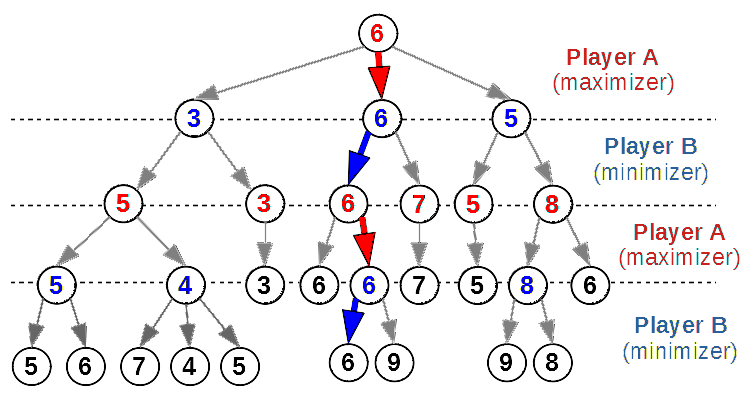
\includegraphics[width=3in]{minimax2.png}}
\caption{\label{fig:minimax2} Minimax in a tree.}
\end{figure}


\vspace{10pt}
{\bf Question 14.} Answer: $6,2$\\
There are $N=6$ steps to go from $P_0$ to $P_6$. 
After that there is a periodic repeat of positions $P_6$ and $P_7$ 
with period $T = 2$ (see Figure~\ref{fig:conway-line5}).


\begin{figure}[!htb]
\center{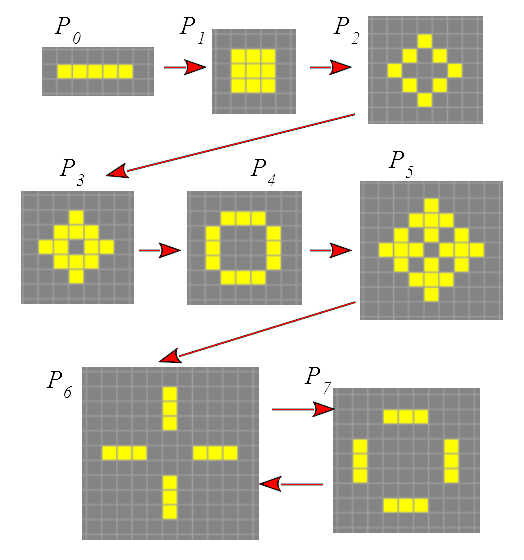
\includegraphics[width=3in]{conway-line5.png}}
\caption{\label{fig:conway-line5} Conway Positions.}
\end{figure}


\vspace{10pt}
{\bf Question 15.} Answer: {\bf (B)}\\

A theory which can prove a statement and its negation is called {\bf not consistent}. 
(On the contrary, theories where this can never happen are called {\bf consistent}).

BTW the first G\"{o}del's Incompleteness Theorem states that any theory about integer numbers that 
is effectively axiomatizable and consistent should also be incomplete 
(i.e.\ there are true results that cannot be proven). So the theory $\mathcal{T}$ from our problem has a chance to 
be complete. But being inconsistent makes it completely useless (if a statement and its negation are
both provable, then virtually anything can be proven, since 
both provable statements $A$ and $\neg A$ also imply 
$(A \wedge \neq A) = \mathtt{false}$. But
such {\tt false} theorem would imply anything \textendash{} whether it makes sense or not.


\vspace{10pt}
{\bf Question 16.} Answer: $4$\\
The full 19-digit credit card number is this: 
$$\mathtt{557367054456450571}\textcolor{red}{\mathtt{4}}.$$

See \url{https://bit.ly/2Y6NaWv} for online Luhn check. 
The procedure is as follows:

\begin{itemize}
\item Drop the last digit from the number. (It is initially unknown in our case.) 
\item Reverse the digits.
\item Multiply the digits in odd positions ($1$, $3$, $5$, etc.) by $2$ and subtract $9$ to all any result higher than $9$. 
\item Add all the obtained numbers together
\item The last (unknown) number is the amount that you would need to add to get a multiple of 10. 
\end{itemize}

\begin{verbatim}
5,5,7,3,6,7,0,5,4,4,5,6,4,5,0,5,7,1 
1,7,5,0,5,4,6,5,4,4,5,0,7,6,3,7,5,5 
2,7,10,0,10,4,12,5,8,4,10,0,14,6,6,7,10,5
2,7,1,0,1,4,3,5,8,4,1,0,5,6,6,7,1,5
\end{verbatim}

The sum of all digits on the last line is $66$. By adding digit $4$ this number becomes divisible by $10$. 






\vspace{10pt}
{\bf Question 17.} Answer {\bf (A)}\\

We should apply our intuition about natural language texts. 
If there are many identical sequences of five consecutive words, then they 
cannot appear by pure chance (there might be some common proverbs or short quotes, 
but they would not make $10\%$ overlap. 

Answer {\bf (B)} is not credible \textendash{} if random lookups in the hashtable lead to $5\%$ matching, 
then $10\%$ overlap cannot be explained by chance.\\
Answer {\bf (C)} is not applicable either; rolling hash on words (especially, if it detects considerable
number of matches) is more useful than rolling hash on characters \textendash{} matching the characters
is less robust and the hash windows are typically shorter. 


\vspace{10pt}
{\bf Question 18.} Answer $30$\\
Truncated icosahedron (soccer ball graph) has the following number of 
faces, edges and vertices:
$$F = 32, E = 90, V = 60.$$

Since Hamilton graph visits all $60$ vertices, 
it should also have $60$ edges. 
For this reason, there are $E - V = 90 - 60 = 30$ edges
that are not part of the Hamiltonian cycle.


\end{document}

